\documentclass[11pt]{article}

\usepackage{amsmath,amssymb,mathtools}
\usepackage[margin=1in]{geometry}
\usepackage{enumitem}
\usepackage{xcolor}
\usepackage{microtype}
\usepackage{graphicx}
\usepackage{tikz,float}
\usepackage{subcaption}
\usepackage{amsthm}
\usepackage{hyperref}
\usepackage{array}
\usepackage{pgfplots}

\usetikzlibrary{shapes.geometric, arrows.meta, positioning, calc, decorations.markings}
\tikzset{
	block/.style={rectangle, draw, text width=6em, text centered, rounded corners, minimum height=10mm},
	sum/.style={circle, draw, node distance=1.5cm},
	line/.style={draw, -{Stealth[length=2.5mm, width=1.5mm]}}
}

\usepgfplotslibrary{groupplots}
\pgfplotsset{compat=1.18}

\pgfplotsset{
	myaxes/.style={
		axis lines=middle,
		axis line style={-latex},
		grid=major,
		grid style={gray!15},
		minor grid style={gray!35},
		xlabel style={at={(ticklabel* cs:1)}, anchor=north west},
		ylabel style={at={(ticklabel* cs:1)}, anchor=south east},
		every axis plot/.append style={thick}
	},
	myplotstyle/.style={
		width=14cm,
		height=7cm,
		axis lines=middle,
		axis line style={-Stealth},
		grid=both,
		minor tick num=1,
		major grid style={draw=gray!30},
		minor grid style={draw=gray!15},
		tick label style={font=\small, fill=white, inner sep=1.5pt},
		xlabel={$t$},
		ylabel={$x(t)$},
		xlabel style={anchor=north east, font=\small},
		ylabel style={anchor=south east, font=\small},
		samples=401,
	}
}

\newtheoremstyle{mynote}
{6pt}      % Space above
{6pt}      % Space below
{}          % Body font (normal, not italic)
{}          % Indent amount
{\bfseries} % Theorem head font
{.}         % Punctuation after theorem head
{.5em}      % Space after theorem head
{}          % Theorem head spec
\theoremstyle{mynote}
\newtheorem{definition}{Definition}
\newtheorem{proposition}{Proposition}
\newtheorem{example}{Example}
\newtheorem{remark}{Remark}
\newtheorem{theorem}{Theorem}
\newtheorem{corollary}{Corollary}

\newcommand{\T}{\mathcal{T}}
\newcommand{\R}{\mathbb{R}}
\newcommand{\Z}{\mathbb{Z}}
\newcommand{\C}{\mathbb{C}}
\newcommand{\conv}{\ast}
\newcommand{\dt}{\,\dd t}
\newcommand{\dd}{\mathrm{d}}
\newcommand{\imp}{\delta}
\newcommand{\sinc}[1]{\frac{\sin(\pi #1)}{\pi #1}}


\DeclareMathOperator{\rect}{rect}
\DeclareMathOperator{\Ev}{Ev}
\DeclareMathOperator{\Od}{Od}
\DeclareMathOperator{\sgn}{sgn}
\DeclareMathOperator{\step}{u}
\DeclareMathOperator{\tri}{tri}


\begin{document}
	% Reset figure counter for this lecture
	\renewcommand{\thefigure}{6.\arabic{figure}}
	
	% --- TITLE BLOCK ---
	\thispagestyle{empty}
	\noindent
	\begin{tabular*}{\textwidth}{l @{\extracolsep{\fill}} r}
		\textbf{Signals and Systems} & \textbf{Lecture 6} \\
		\textit{Dr. Ghandi Manasra and Ahmed Rabei} & \textit{Fall 2025} \\
	\end{tabular*}
	\hrule
	\vspace{0.4cm}
	\begin{center}
		\Large\textbf{Lecture 6: LTI Properties and Equation-Described Systems}
	\end{center}
	\vspace{0.4cm}
	
\section*{Reference}
	Oppenheim \& Willsky, \textit{Signals and Systems}, Chapter 2, Sections 2.3--2.4

\section*{Review of Lecture 5}
	\begin{itemize}[noitemsep]
		\item Convolution integral for CT systems
		\item Flip-and-slide method for computing convolution
		\item Physical examples of convolution
	\end{itemize}

\section*{6.1 Introduction}

The core result from last time is the convolution representation:
\[
y(t) = x(t) \conv h(t) = \int_{-\infty}^{\infty} x(\tau)h(t-\tau) \dd\tau
\]
\[
y[n] = x[n] \conv h[n] = \sum_{k=-\infty}^{\infty} x[k] h[n-k]
\]

Today, those formulas become a tool to analyze memory, invertibility, causality, and stability purely from $h$, and to connect to systems given by constant-coefficient differential and difference equations.

\section*{6.2 Convolution Properties}

The convolution operation has several crucial algebraic properties that define the structure of LTI systems.

\subsection*{6.2.1 Commutative Property}

Convolution is commutative. The roles of the input and the impulse response are interchangeable.
\[
x(t) \conv h(t) = h(t) \conv x(t), \qquad x[n] \conv h[n] = h[n] \conv x[n]
\]

\textbf{Intuition:} You can flip and slide either $x(t)$ or $h(t)$ and get the same result.

\subsection*{6.2.2 Distributive Property}

Convolution distributes over addition. 
\[
x(t) \conv (h_1(t) + h_2(t)) = x(t) \conv h_1(t) + x(t) \conv h_2(t)
\]

\textbf{Intuition:} The response to two LTI systems in parallel is the same as the response to a single system whose impulse response is the sum of the two individual impulse responses.

\subsection*{6.2.3 Associative Property}

Convolution is associative. 
\[
(x(t) \conv h_1(t)) \conv h_2(t) = x(t) \conv (h_1(t) \conv h_2(t))
\]

\textbf{Intuition:} The overall impulse response of a cascade of LTI systems is the convolution of the individual impulse responses. For LTI systems, the \textbf{order of the cascade does not matter}.

\begin{remark}
The commutativity and associativity of LTI systems is a very special and powerful property. This is NOT true for nonlinear systems. A classic example: A "square" block followed by an "add 3" block gives $(x^2)+3$. Reversing the order gives $(x+3)^2$, which is completely different.
\end{remark}

\subsection*{6.2.4 Demonstration: Commutative Property}

\begin{figure}[H]
	\centering
	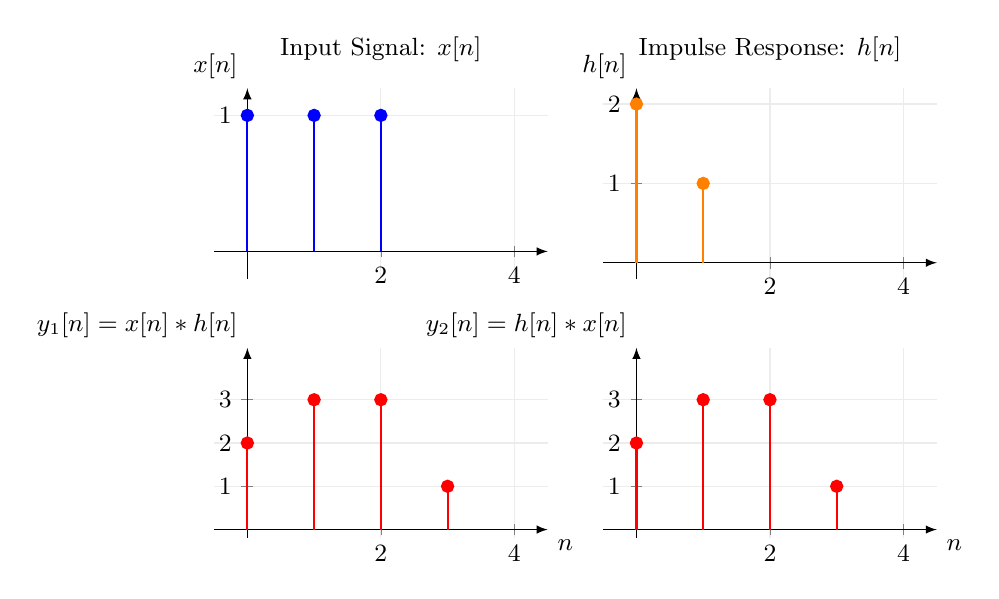
\begin{tikzpicture}
	\begin{groupplot}[
		group style={group size=2 by 2, horizontal sep=20pt, vertical sep=25pt},
		/tikz/font=\small,
		width=0.48\linewidth, height=4cm,
		myaxes, % A custom style for axes, define it in your preamble
		ymin=-0.2, xmin=-0.5, xmax=4.5,
		samples at={-1,...,5}
		]
		
		% Plot 1: Input signal x[n]
		\nextgroupplot[
		title={Input Signal: $x[n]$},
		ylabel={$x[n]$}, ymax=1.2, ytick={0,1}
		]
		\addplot[ycomb, mark=*, thick, blue] coordinates {
			(0,1) (1,1) (2,1)
		};
		
		% Plot 2: Impulse response h[n]
		\nextgroupplot[
		title={Impulse Response: $h[n]$},
		ylabel={$h[n]$}, ymax=2.2, ytick={0,1,2}
		]
		\addplot[ycomb, mark=*, thick, orange] coordinates {
			(0,2) (1,1)
		};
		
		% Plot 3: Convolution y[n] = x[n] * h[n]
		\nextgroupplot[
		ylabel={ $y_1[n] = x[n] * h[n]$}, ymax=4.2, ytick={0,1,2,3},
		xlabel={$n$}
		]
		\addplot[ycomb, mark=*, thick, red] coordinates {
			(0,2) (1,3) (2,3) (3,1)
		};
		
		% Plot 4: Convolution y[n] = h[n] * x[n]
		\nextgroupplot[
		ylabel={$y_2[n] = h[n] * x[n]$}, ymax=4.2, ytick={0,1,2,3},
		xlabel={$n$}
		]
		\addplot[ycomb, mark=*, thick, red] coordinates {
			(0,2) (1,3) (2,3) (3,1)
		};
		
	\end{groupplot}
\end{tikzpicture}
	\caption{Commutative property of convolution: $x[n] * h[n] = h[n] * x[n]$.}
	\label{fig:convolution_properties}
\end{figure}

\subsection*{6.2.5 Convolution with Sparse Impulse Responses}

If $h[n] = \sum_k c_k \imp[n-n_k]$, then:
\[
y[n] = \sum_k c_k x[n-n_k]
\]

Convolution becomes a weighted sum of delayed copies, modeling echoes and multipath channels.

\newpage

\section*{6.3 Correlation Functions}

Correlation provides a measure of similarity or dissimilarity between two signals. It is a fundamental tool in signal processing for pattern recognition, synchronization, and noise analysis.

\subsection*{6.3.1 Cross-Correlation Function}

The cross-correlation function measures the similarity between two different signals as one is shifted relative to the other.

\textbf{Continuous-Time:}
\[
R_{xy}(t) = \int_{-\infty}^{\infty} x(\tau) y(\tau + t) \dd\tau = \int_{-\infty}^{\infty} x(\tau - t) y(\tau) \dd\tau
\]

\textbf{Discrete-Time:}
\[
R_{xy}[n] = \sum_{k=-\infty}^{\infty} x[k] y[k + n] = \sum_{k=-\infty}^{\infty} x[k - n] y[k]
\]

\textbf{Key Properties:}
\begin{itemize}[noitemsep]
	\item $R_{xy}(t) = R_{yx}(-t)$ (order matters)
	\item $|R_{xy}(t)| \leq \sqrt{R_{xx}(0) R_{yy}(0)}$ (Cauchy-Schwarz inequality)
	\item If signals are uncorrelated: $R_{xy}(t) \approx 0$ for all $t$
\end{itemize}

\subsection*{6.3.2 Autocorrelation Function}

The autocorrelation function measures how much a signal matches a delayed version of itself.

\textbf{Continuous-Time:}
\[
R_{xx}(t) = \int_{-\infty}^{\infty} x(\tau) x(\tau + t) \dd\tau = \int_{-\infty}^{\infty} x(\tau - t) x(\tau) \dd\tau
\]

\textbf{Discrete-Time:}
\[
R_{xx}[n] = \sum_{k=-\infty}^{\infty} x[k] x[k + n] = \sum_{k=-\infty}^{\infty} x[k - n] x[k]
\]

\textbf{Key Properties:}
\begin{itemize}[noitemsep]
	\item $R_{xx}(t) = R_{xx}(-t)$ (even function)
	\item $R_{xx}(0) \geq |R_{xx}(t)|$ for all $t$ (maximum at zero lag)
	\item $R_{xx}(0) = \int_{-\infty}^{\infty} |x(\tau)|^2 \dd\tau$ (total energy)
\end{itemize}

\subsection*{6.3.3 Normalized Correlation Function}

The normalized correlation function $\rho_{xy}(t)$ provides a measure of similarity that is independent of signal amplitude, ranging from -1 to +1. This technique is crucial for detecting known signals or patterns within larger signals, especially when signal energy or power is unknown or varies.

The foundation is the cross-correlation function. However, the magnitude of $R_{xy}(t)$ depends on signal amplitudes. If you double the amplitude of both signals, the cross-correlation value quadruples, even though their shape similarity remains unchanged.To overcome this amplitude dependency, we use normalized correlation. The denominator is the geometric mean of the signal energies.

\textbf{Continuous-Time:}
\[
\rho_{xy}(t) = \frac{R_{xy}(t)}{\sqrt{R_{xx}(0) R_{yy}(0)}} = \frac{\int_{-\infty}^{\infty} x(\tau) y(\tau + t) \dd\tau}{\sqrt{\int_{-\infty}^{\infty} |x(\tau)|^2 \dd\tau \int_{-\infty}^{\infty} |y(\tau)|^2 \dd\tau}}
\]

\textbf{Discrete-Time:}
\[
\rho_{xy}[n] = \frac{R_{xy}[n]}{\sqrt{R_{xx}[0] R_{yy}[0]}} = \frac{\sum_{k=-\infty}^{\infty} x[k] y[k + n]}{\sqrt{\sum_{k=-\infty}^{\infty} |x[k]|^2 \sum_{k=-\infty}^{\infty} |y[k]|^2}}
\]

\textbf{Key Properties:}
\begin{itemize}[noitemsep]
	\item $-1 \leq \rho_{xy}(t) \leq +1$ for all $t$ (bounded range)
	\item $\rho_{xy}(t) = +1$ when $y(t) = kx(t)$ for $k > 0$ (perfect positive correlation)
	\item $\rho_{xy}(t) = -1$ when $y(t) = kx(t)$ for $k < 0$ (perfect negative correlation)
	\item $\rho_{xy}(t) = 0$ when signals are uncorrelated (orthogonal)
	\item $\rho_{xx}(t) = 1$ at $t = 0$ and $|\rho_{xx}(t)| \leq 1$ for all $t$
\end{itemize}

\textbf{Key takeaways:}

The normalized correlation coefficient $\rho_{xy}(t)$ always lies in the range of \textbf{-1 to +1}:

\begin{itemize}[noitemsep]
	\item \textbf{$\rho_{xy}(t) = +1$:} Perfect positive correlation at time lag $t$. The two signals are identical in shape, and one may be a positive scaled version of the other.
	\item \textbf{$\rho_{xy}(t) = -1$:} Perfect negative correlation at time lag $t$. The signals have the exact same shape, but one is inverted (a negative scaled version of the other).
	\item \textbf{$\rho_{xy}(t) = 0$:} No correlation between the signals at that specific time lag. They are considered orthogonal.
	\item \textbf{Values between 0 and 1:} Indicate a degree of positive similarity. The closer to 1, the more similar the signals are.
	\item \textbf{Values between -1 and 0:} Suggest a degree of negative similarity. The closer to -1, the more they are alike in shape but opposite in sign.
\end{itemize}

\begin{example}[Normalized Cross-Correlation]
For $x(t) = e^{-t}u(t)$ and $y(t) = 2e^{-t}u(t)$, find $\rho_{xy}(t)$.

\textbf{Solution:}
First, compute the autocorrelations:
\[
R_{xx}(0) = \int_0^{\infty} e^{-2\tau} \dd\tau = \frac{1}{2}, \quad R_{yy}(0) = \int_0^{\infty} 4e^{-2\tau} \dd\tau = 2
\]

The cross-correlation is:
\[
R_{xy}(t) = \int_0^{\infty} e^{-\tau} \cdot 2e^{-(\tau+t)} \dd\tau = 2e^{-t} \int_0^{\infty} e^{-2\tau} \dd\tau = e^{-t}
\]

Therefore:
\[
\rho_{xy}(t) = \frac{e^{-t}}{\sqrt{\frac{1}{2} \cdot 2}} = e^{-t}
\]

This shows perfect positive correlation at $t = 0$ ($\rho_{xy}(0) = 1$) that decays exponentially.
\end{example}
\newpage
\textbf{Key Applications:}


\begin{itemize}[noitemsep]
	\item \textbf{Pattern Recognition and Template Matching:} A known "template" signal is correlated with a larger signal to find occurrences of the template. For example, in image processing, it can find specific objects regardless of lighting conditions (which affect amplitude).
	\item \textbf{Radar and Sonar Systems:} Used to detect returned signals (echoes) in the presence of noise. By correlating the received signal with the transmitted pulse, the system can determine distance to objects.
	\item \textbf{Communications:} Helps synchronize receivers with incoming signals and detect specific bit sequences in digital communications.
	\item \textbf{Biomedical Signal Processing:} Identifies specific patterns in physiological signals like ECGs or EEGs that might indicate medical conditions.
	\item \textbf{Feature Detection:} Provides robust similarity measures unaffected by signal amplitude variations.
\end{itemize}


\subsection*{6.3.4 Relationship Between Correlation and Convolution}

Correlation and convolution are closely related. For cross-correlation:
\[
R_{xy}(t) = x(t) * y(-t)
\]

This means correlation can be computed using convolution by time-reversing one of the signals.

\textbf{Proof:}
\begin{align}
x(t) * y(-t) &= \int_{-\infty}^{\infty} x(\tau) y(-(t-\tau)) \dd\tau \\
&= \int_{-\infty}^{\infty} x(\tau) y(\tau - t) \dd\tau \\
&= R_{xy}(t)
\end{align}

\subsection*{6.3.5 Examples and Applications}

\begin{example}[Autocorrelation of Exponential Signal]
For $x(t) = 2e^{-3t}u(t)$, find $R_{xx}(t)$.

\textbf{Solution:}
For $t > 0$:
\[
R_{xx}(t) = \int_0^{\infty} (2e^{-3\tau})(2e^{-3(\tau+t)}) \dd\tau = 4e^{-3t} \int_0^{\infty} e^{-6\tau} \dd\tau = \frac{2}{3}e^{-3t}
\]

For $t < 0$:
\[
R_{xx}(t) = \int_{-t}^{\infty} (2e^{-3\tau})(2e^{-3(\tau+t)}) \dd\tau = \frac{2}{3}e^{3t}
\]

Therefore: $R_{xx}(t) = \frac{2}{3}e^{-3|t|}$ for all $t$.
\end{example}

\begin{example}[Cross-Correlation of Rectangular Pulses]
For $x(t) = u(t) - u(t-1)$ and $y(t) = u(t-\frac{3}{2}) - u(t-\frac{5}{2})$, find $R_{xy}(t)$.

The cross-correlation shows the overlap between the two rectangular pulses as one slides past the other, with maximum correlation when they align.
\end{example}

\subsection*{6.3.6 Periodic Signals (Power Signals)}

For periodic signals with period $T$ (CT) or $N$ (DT), correlation functions are also periodic:

\textbf{Continuous-Time:}
\[
R_{xy}(t) = \frac{1}{T} \int_0^T x(\tau) y(\tau + t) \dd\tau
\]

\textbf{Discrete-Time:}
\[
R_{xy}[n] = \frac{1}{N} \sum_{k=0}^{N-1} x[k] y[k + n]
\]

For periodic signals, $R_{xx}(0)$ represents the average power rather than total energy.

\section*{6.4 System Properties via the Impulse Response}

We can now connect the system properties from Lecture 3 to specific conditions on the impulse response $h(t)$ or $h[n]$.

\subsection*{6.4.1 Memoryless Systems}

An LTI system is \textbf{memoryless} if and only if its impulse response is a scaled impulse.
\[
h(t) = K\imp(t) \quad \text{or} \quad h[n] = K\imp[n]
\]

The system's output can only depend on the current input if the impulse response itself is zero everywhere except at time zero.

\subsection*{6.4.2 Invertible Systems}

An LTI system is \textbf{invertible} if we can find an inverse system, $h_{inv}(t)$, that recovers the original input. This means:
\[
h(t) \conv h_{inv}(t) = \imp(t) \quad \text{or} \quad h[n] \conv h_{inv}[n] = \imp[n]
\]

Practically, noninvertibility arises from nonminimum-phase zeros or spectral nulls that annihilate components of inputs.

\subsection*{6.4.3 Causal Systems}

An LTI system is \textbf{causal} if and only if its impulse response is zero for all negative time.
\[
h(t) = 0 \text{ for } t < 0 \quad \text{and} \quad h[n] = 0 \text{ for } n < 0
\]

The system cannot respond to an impulse before the impulse is applied. The convolution integral for a causal system simplifies to:
\[
y(t) = \int_{-\infty}^{t} x(\tau)h(t-\tau)\dd\tau, \qquad y[n] = \sum_{k=0}^{\infty} h[k] x[n-k]
\]

\subsubsection*{Demonstration: Causality Analysis}

\begin{figure}[H]
	\centering
	\begin{figure}[H]
	\centering
	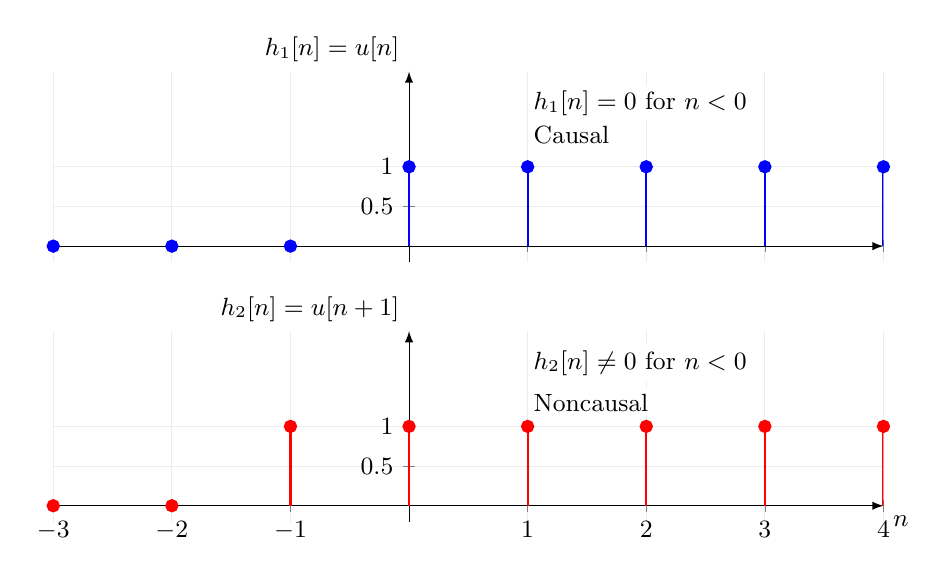
\begin{tikzpicture}
		\begin{groupplot}[
			group style={group size=1 by 2, vertical sep=25pt, xticklabels at=edge bottom},
			/tikz/font=\small,
			width=\linewidth, height=4cm, myaxes,
			xmin=-3, xmax=4,
			samples at={-3,...,4}]
			
			\nextgroupplot[ylabel={$h_1[n] = u[n]$}, ymin=-0.2, ymax=2.2, ytick={0,0.5,1}, title={}]
			\addplot[ycomb, mark=*, thick, blue] coordinates {
				(-3,0) (-2,0) (-1,0) (0,1) (1,1) (2,1) (3,1) (4,1)
			};
			\node[anchor=west, fill=white, inner sep=2pt] at (axis cs:1,1.8) 
			{$h_1[n] = 0$ for $n < 0$};
			\node[anchor=west, fill=white, inner sep=2pt] at (axis cs:1,1.4) 
			{Causal};
			
			\nextgroupplot[xlabel={$n$}, ylabel={$h_2[n] = u[n+1]$}, ymin=-0.2, ymax=2.2, ytick={0,0.5,1}, title={}]
			\addplot[ycomb, mark=*, thick, red] coordinates {
				(-3,0) (-2,0) (-1,1) (0,1) (1,1) (2,1) (3,1) (4,1)
			};
			\node[anchor=west, fill=white, inner sep=2pt] at (axis cs:1,1.8) 
			{$h_2[n] \neq 0$ for $n < 0$};
			\node[anchor=west, fill=white, inner sep=2pt] at (axis cs:1,1.3) 
			{Noncausal};
		\end{groupplot}
	\end{tikzpicture}
\end{figure}

	\caption{Causal vs noncausal systems based on impulse response.}
	\label{fig:causality_examples}
\end{figure}

\subsection*{6.4.4 BIBO Stable Systems}

An LTI system is \textbf{stable} if and only if its impulse response is \textbf{absolutely integrable} (CT) or \textbf{absolutely summable} (DT).
\[
\int_{-\infty}^{\infty} |h(t)| \dd t < \infty \quad \text{and} \quad \sum_{n=-\infty}^{\infty} |h[n]| < \infty
\]

\begin{remark}
Once the system is described by h(t), properties like causality, memorylessness, invertibility, and stability can be checked directly from h(t) without further ambiguity; for stability in particular, the tail of h(t) must decay so that the total "effect" of past inputs remains finite.
\end{remark}

\subsection*{6.4.5 Demonstration: Stability Analysis}

\begin{figure}[H]
	\centering
	\begin{figure}[H]
	\centering
	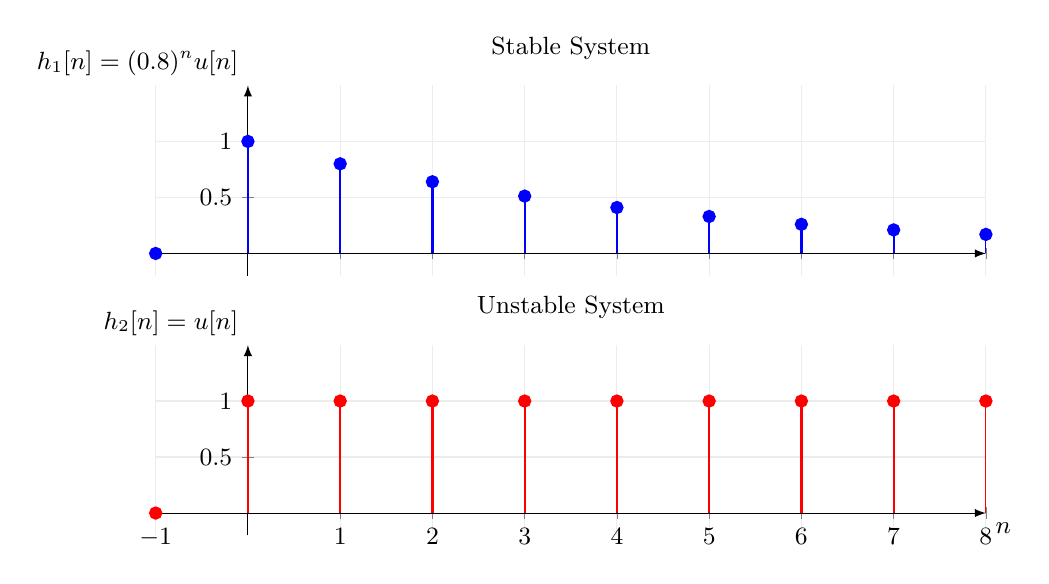
\begin{tikzpicture}
	\begin{groupplot}[
		group style={group size=1 by 2, vertical sep=25pt, xticklabels at=edge bottom},
		/tikz/font=\small,
		width=\linewidth, height=4cm, myaxes,
		xmin=-1, xmax=8,
		samples at={-1,...,8}]
		
		\nextgroupplot[ylabel={$h_1[n] = (0.8)^n u[n]$}, ymin=-0.2, ymax=1.5, ytick={0,0.5,1}, title={Stable System}]
		\addplot[ycomb, mark=*, thick, blue] coordinates {
			(-1,0) (0,1) (1,0.8) (2,0.64) (3,0.512) (4,0.41) (5,0.33) (6,0.26) (7,0.21) (8,0.17)
		};
	
		
		\nextgroupplot[xlabel={$n$}, ylabel={$h_2[n] = u[n]$}, ymin=-0.2, ymax=1.5, ytick={0,0.5,1}, title={Unstable System}]
		\addplot[ycomb, mark=*, thick, red] coordinates {
			(-1,0) (0,1) (1,1) (2,1) (3,1) (4,1) (5,1) (6,1) (7,1) (8,1)
		};

	\end{groupplot}
	\end{tikzpicture}
\end{figure}

	\caption{Stable vs unstable systems based on impulse response properties.}
	\label{fig:stability_examples}
\end{figure}

\textbf{Stable System:} $h[n] = (0.8)^n u[n]$
\[
\sum_{n=0}^{\infty} |0.8^n| = \frac{1}{1-0.8} = 5 < \infty \quad \text{(Stable)}
\]\\
\textbf{Unstable System:} Accumulator $h[n] = u[n]$
\[
\sum_{n=0}^{\infty} |1| = \infty \quad \text{(Unstable)}
\]

\section*{6.5 Step Response and Recovering the Impulse Response}

\subsection*{6.5.1 Discrete-Time Case}

With step input $u[n]$ and step response $s[n] = h[n] \conv u[n]$, we can recover $h$ via first difference:
\[
h[n] = s[n] - s[n-1] \quad \text{for all } n
\]

\subsection*{6.5.2 Continuous-Time Case}

With step input $u(t)$ and step response $s(t) = h(t) \conv u(t)$, we can recover $h$ via differentiation:
\[
h(t) = \frac{\dd}{\dd t} s(t)
\]

For causal LTI systems, $s(t) = \int_0^t h(\tau) \dd\tau$ and differentiability almost everywhere yields $h$.

\section*{6.6 Systems Described by Differential and Difference Equations}

This is the most important and practical class of LTI systems in engineering applications.

\subsection*{6.6.1 Linear Constant-Coefficient Differential Equations (CT)}

The general form is:
\[
\sum_{k=0}^{N} a_k \frac{\dd^k y(t)}{\dd t^k} = \sum_{k=0}^{M} b_k \frac{\dd^k x(t)}{\dd t^k}
\]
where $a_k$ and $b_k$ are constants, and $N$ is the order of the system.

\subsubsection*{Solution Structure and Auxiliary Conditions}

The solution $y(t)$ consists of two parts:
\[
y(t) = y_h(t) + y_p(t)
\]
where:
\begin{itemize}[noitemsep]
	\item $y_h(t)$ is the \textbf{homogeneous solution} (natural response)
	\item $y_p(t)$ is the \textbf{particular solution} (forced response)
\end{itemize}

\textbf{Critical Requirements:}
\begin{enumerate}[noitemsep]
	\item The differential equation alone does not completely specify the output in terms of the input.
	\item We need \textbf{auxiliary conditions} corresponding to the values of $y(t)$ and its first $(N-1)$ derivatives at some point in time.
	\item For the system to be \textbf{linear}, all auxiliary conditions must be \textbf{zero}.
	\item For the system to be \textbf{causal and LTI}, we must assume \textbf{initial rest}.
\end{enumerate}

\subsubsection*{Initial Rest Condition}

\textbf{Definition:} If $x(t) = 0$ for $t \leq t_0$, then $y(t) = 0$ for $t \leq t_0$.

Under initial rest, the response for $t > t_0$ can be calculated from the differential equation with initial conditions:
\[
y(t_0) = \frac{\dd y(t_0)}{\dd t} = \cdots = \frac{\dd^{N-1}y(t_0)}{\dd t^{N-1}} = 0
\]

This ensures the system is \textbf{causal, linear, and time-invariant}.

\subsubsection*{Normalized Form}

When $M = N$, we can write:
\[
y(t) = \frac{1}{a_0}\left[\sum_{k=0}^{N} b_k \frac{\dd^k x(t)}{\dd t^k} - \sum_{k=1}^{N} a_k \frac{\dd^k y(t)}{\dd t^k}\right]
\]

This form is particularly useful for implementation and analysis.

\begin{example}[RC Circuit]
Consider the first-order RC circuit:
\[
RC\frac{\dd y}{\dd t} + y = x
\]
With initial rest, this gives:
\[
h(t) = \frac{1}{RC}e^{-t/(RC)}u(t)
\]
This system is causal, stable, and has step response $1 - e^{-t/(RC)}$.
\end{example}

\subsection*{6.6.2 Linear Constant-Coefficient Difference Equations (DT)}

The general form is:
\[
\sum_{k=0}^{N} a_k y[n-k] = \sum_{k=0}^{M} b_k x[n-k]
\]

\subsubsection*{Initial Rest Condition (DT)}

For the system to be \textbf{causal and LTI}, we must assume \textbf{initial rest}:
\begin{itemize}[noitemsep]
	\item If $x[n] = 0$ for $n \leq n_0$, then $y[n] = 0$ for $n \leq n_0$.
	\item This ensures the system has no "memory" of past inputs before the input begins.
	\item Under initial rest, the system is causal, linear, and time-invariant.
\end{itemize}

\subsubsection*{Solution Structure and Properties}

The solution approach is analogous to differential equations, but with an alternative recursive form:
\[
y[n] = \frac{1}{a_0}\left[\sum_{k=0}^{M} b_k x[n-k] - \sum_{k=1}^{N} a_k y[n-k]\right]
\]

\textbf{Key Properties:}
\begin{enumerate}[noitemsep]
	\item The difference equation alone does not completely specify the output.
	\item For linearity, auxiliary conditions must be zero.
	\item If $N \geq 1$: \textbf{Infinite Impulse Response (IIR)} system.
	\item If $N = 0$: \textbf{Finite Impulse Response (FIR)} system.
\end{enumerate}

\subsubsection*{FIR vs IIR Systems}

\textbf{FIR System ($N = 0$):}
\[
y[n] = \sum_{k=0}^{M} \frac{b_k}{a_0}x[n-k]
\]

Impulse response:
\[
h[n] = \begin{cases}
\frac{b_k}{a_0} & 0 \leq n \leq M \\
0 & \text{otherwise}
\end{cases}
\]

\textbf{IIR System ($N \geq 1$):}
\begin{itemize}[noitemsep]
	\item Has infinite-length impulse response
	\item Output depends on past output values
	\item More complex but more powerful
\end{itemize}

\subsubsection*{Cascade Interpretation}

For $M = N$, the difference equation can be interpreted as a cascade of two systems:

\textbf{Nonrecursive (FIR) part:}
\[
w[n] = \sum_{k=0}^{N} b_k x[n-k]
\]

\textbf{Recursive (IIR) part:}
\[
y[n] = \frac{1}{a_0}\left[w[n] - \sum_{k=1}^{N} a_k y[n-k]\right]
\]

\begin{example}[Moving Average Filter]
Consider the 4-point moving average:
\[
y[n] = \frac{1}{4}(x[n] + x[n-1] + x[n-2] + x[n-3])
\]
This is an FIR system with impulse response:
\[
h[n] = \frac{1}{4}(\imp[n] + \imp[n-1] + \imp[n-2] + \imp[n-3])
\]
\end{example}

\begin{example}[First-Order IIR Filter]
Consider the recursive filter:
\[
y[n] = \alpha y[n-1] + (1-\alpha) x[n]
\]
This is an IIR system with impulse response:
\[
h[n] = (1-\alpha) \alpha^n u[n]
\]
For $|\alpha| < 1$, the system is stable.
\end{example}

\section*{6.7 Implementation Structures}

The normalized forms of LCCDEs can be implemented using block diagrams. Two common structures are:

\subsection*{6.7.1 Direct Form I}

This structure directly implements the cascade interpretation:
\begin{itemize}[noitemsep]
	\item First: Nonrecursive (feedforward) section
	\item Second: Recursive (feedback) section
	\item Uses separate delay chains for input and output
	\item Maps closely to the equation coefficients
	\item Intuitive for understanding
\end{itemize}
\vspace*{\fill}
\subsection*{6.7.2 Direct Form II}

This structure reverses the order and shares the delay chain:
\begin{itemize}[noitemsep]
	\item First: Recursive section with shared delays
	\item Second: Nonrecursive section
	\item More efficient in terms of memory usage
	\item Practical for embedded DSP designs
	\item Requires careful numerical conditioning
\end{itemize}

\begin{figure}[htbp]
	\centering
\resizebox{0.8\textwidth}{!}{		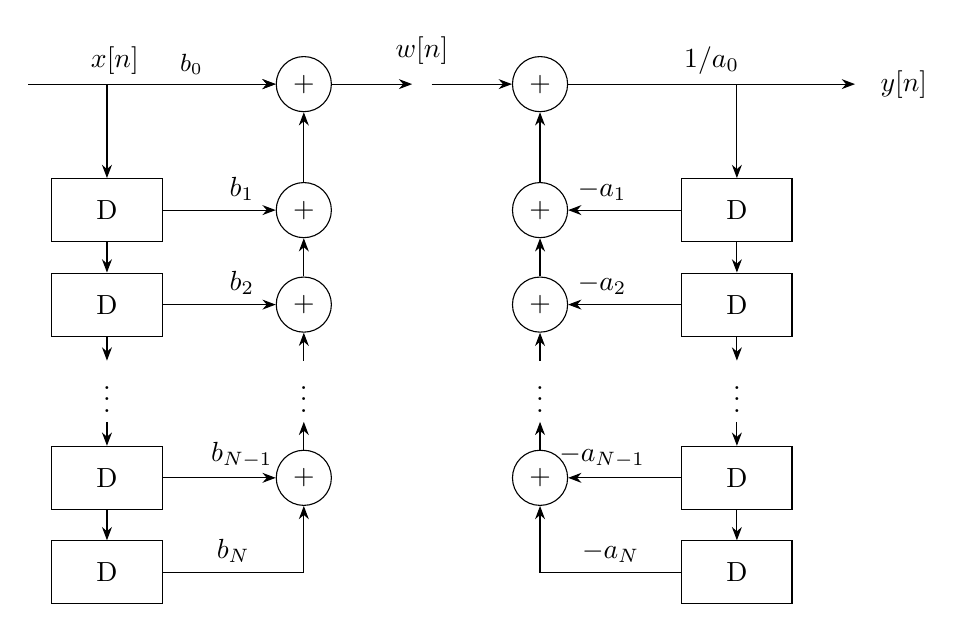
\begin{tikzpicture}[
	node distance=8mm and 18mm,
	block/.style={rectangle, draw, minimum width=14mm, minimum height=8mm, align=center},
	sum/.style={circle, draw, minimum size=7mm, inner sep=0pt},
	coeff/.style={font=\small},
	>={Stealth}
	]
	
	% Main horizontal nodes
	\coordinate (input) at (0,0);
	\node[sum] (feedforward_sum) at (3.5,0) {$+$};
	\node (intermediate_signal) at (5,0) [label=above:{$w[n]$}] {};
	\node[sum] (feedback_sum) at (6.5,0) {$+$};
	\coordinate (output) at (10.5,0);
	
	% Main path arrows and labels
	\draw[->] (input) -- node[above,pos=0.35] {$x[n]$} (feedforward_sum);
	\draw[->] (feedforward_sum) -- (intermediate_signal);
	\draw[->] (intermediate_signal) -- (feedback_sum);
	\draw[->] (feedback_sum) -- node[above] {$1/a_0$} (output) node[right=2mm] {$y[n]$};
	
	%
	% Feedforward column (left)
	%
	% a vertical bus point where taps branch off
	\coordinate (feedforward_bus) at (1,0);
	
	% delays stacked below ffbus
	\node[block] (delay_1) at ($(feedforward_bus)+(0,-1.6)$) {D};
	\node[block] (delay_2) at ($(delay_1)+(0,-1.2)$) {D};
	\node (delay_dots) at ($(delay_2)+(0,-1.1)$) {$\vdots$};
	\node[block] (delay_N_minus_1) at ($(delay_dots)+(0,-1.1)$) {D};
	\node[block] (delay_N) at ($(delay_N_minus_1)+(0,-1.2)$) {D};
	
	% feedforward bus line and branch to ffsum
	\draw (feedforward_bus) -- ++(0.8,0); % small visual bus
	\draw[->] (feedforward_bus) -- node[above,pos=0.5,coeff] {$b_0$} (feedforward_sum);
	
	% connect the bus to first delay
	\draw[->] (feedforward_bus) -- (delay_1.north);
	
	% chain delays
	\draw[->] (delay_1) -- (delay_2);
	\draw[->] (delay_2) -- (delay_dots);
	\draw[->] (delay_dots) -- (delay_N_minus_1);
	\draw[->] (delay_N_minus_1) -- (delay_N);
	
	% summers for each delayed tap
	\node[sum] (sum_1) at ($(feedforward_sum) + (0,-1.6)$) {$+$};
	\node[sum] (sum_2) at ($(sum_1) + (0,-1.2)$) {$+$};
	\node (sum_dots) at ($(sum_2) + (0,-1.1)$) {$\vdots$};
	\node[sum] (sum_N_minus_1) at ($(sum_dots) + (0,-1.1)$) {$+$};
	
	% connections from delays to the corresponding summers
	\draw[->] (delay_1) -- node[above, pos=0.7] {$b_1$} (sum_1);
	\draw[->] (delay_2) -- node[above, pos=0.7] {$b_2$} (sum_2);
	\draw[->] (delay_N_minus_1) -- node[above, pos=0.7] {$b_{N-1}$} (sum_N_minus_1);
	\draw[->] (delay_N) -| (sum_N_minus_1) node[above, pos=0.25] {$b_N$};
	
	% chain the summers into ffsum
	\draw[->] (sum_1) -- (feedforward_sum);
	\draw[->] (sum_2) -- (sum_1);
	\draw[->] (sum_N_minus_1) -- (sum_dots);
	\draw[->] (sum_dots) -- (sum_2);
	
	%
	% Feedback column (right)
	%
	\coordinate (feedback_bus) at (9,0);
	
	\node[block] (feedback_delay_1) at ($(feedback_bus)+(0,-1.6)$) {D};
	\node[block] (feedback_delay_2) at ($(feedback_delay_1)+(0,-1.2)$) {D};
	\node (feedback_delay_dots) at ($(feedback_delay_2)+(0,-1.1)$) {$\vdots$};
	\node[block] (feedback_delay_N_minus_1) at ($(feedback_delay_dots)+(0,-1.1)$) {D};
	\node[block] (feedback_delay_N) at ($(feedback_delay_N_minus_1)+(0,-1.2)$) {D};
	
	% bus line and chain
	\draw (feedback_bus) -- ++(-0.8,0); % small visual bus
	\draw[->] (feedback_bus) -- (feedback_delay_1.north);
	\draw[->] (feedback_delay_1) -- (feedback_delay_2);
	\draw[->] (feedback_delay_2) -- (feedback_delay_dots);
	\draw[->] (feedback_delay_dots) -- (feedback_delay_N_minus_1);
	\draw[->] (feedback_delay_N_minus_1) -- (feedback_delay_N);
	
	% feedback summers
	\node[sum] (feedback_sum_1) at ($(feedback_sum) + (0,-1.6)$) {$+$};
	\node[sum] (feedback_sum_2) at ($(feedback_sum_1) + (0,-1.2)$) {$+$};
	\node (feedback_sum_dots) at ($(feedback_sum_2) + (0,-1.1)$) {$\vdots$};
	\node[sum] (feedback_sum_N_minus_1) at ($(feedback_sum_dots) + (0,-1.1)$) {$+$};
	
	% connections from feedback delays to feedback summers (with -a_i)
	\draw[->] (feedback_delay_1) -- node[above, pos=0.7] {$-a_1$} (feedback_sum_1);
	\draw[->] (feedback_delay_2) -- node[above, pos=0.7] {$-a_2$} (feedback_sum_2);
	\draw[->] (feedback_delay_N_minus_1) -- node[above, pos=0.7] {$-a_{N-1}$} (feedback_sum_N_minus_1);
	\draw[->] (feedback_delay_N) -| (feedback_sum_N_minus_1) node[above, pos=0.25] {$-a_N$};
	
	% chain feedback summers into main feedback summer
	\draw[->] (feedback_sum_1) -- (feedback_sum);
	\draw[->] (feedback_sum_2) -- (feedback_sum_1);
	\draw[->] (feedback_sum_N_minus_1) -- (feedback_sum_dots);
	\draw[->] (feedback_sum_dots) -- (feedback_sum_2);
	
	
	\end{tikzpicture}}
	\caption{Direct Form I implementation structure for LCCDEs.}
	\label{fig:direct_form_i}
\end{figure}
\vspace*{\fill}

\vspace*{\fill}
\begin{figure}[H]
	\centering
	\resizebox{0.7\textwidth}{!}{	\begin{tikzpicture}[
		node distance=10mm and 22mm,
		block/.style={rectangle, draw, minimum width=12mm, minimum height=8mm, align=center},
		sum/.style={circle, draw, minimum size=7mm, inner sep=0pt},
		>={Stealth},
		% Style for placing labels on lines
		coeff/.style={above, pos=0.5}
		]
		
		% --- Main Horizontal Nodes at the Top ---
		\coordinate (input) at (0,0);
		\node[sum] (feedback_sum_top) at (2.5,0) {$+$};
		\coordinate (w_point) at (5,0);
		\node[sum] (feedforward_sum_top) at (7.5,0) {$+$};
		\coordinate (output) at (10,0);
		
		% --- Draw the Top-Level Signal Path ---
		\draw[->] (input) -- node[coeff, pos=0.4] {$x[n]$} (feedback_sum_top);
		\draw[->] (feedback_sum_top) -- (w_point);
		\node[above=2mm] at (w_point) {$w[n]$};
		\draw[->] (w_point) -- node[coeff] {$b_0$} (feedforward_sum_top);
		\draw[->] (feedforward_sum_top) -- node[coeff, pos=0.6] {$y[n]$} (output);
		
		% --- Central Delay Column ---
		\node[block] (delay1) at ($(w_point)+(0,-2.2)$) {D};
		\node[block] (delay2) at ($(delay1)+(0,-2.2)$) {D};
		\node (dots) at ($(delay2)+(0,-1.8)$) {$\vdots$};
		\node[block] (delayN_1) at ($(dots)+(0,-1.8)$) {D};
		\node[block] (delayN) at ($(delayN_1)+(0,-2.2)$) {D};
		
		% --- Vertical Delay Bus ---
		\draw[->] (w_point) -- (delay1);
		\draw[->] (delay1) -- (delay2);
		\draw[->,shorten >=1mm, shorten <=1mm] (delay2) -- (dots);
		\draw[->,shorten >=1mm, shorten <=1mm] (dots) -- (delayN_1);
		\draw[->] (delayN_1) -- (delayN);
		
		% --- Summers on Both Sides ---
		\node[sum] (feedback_sum_1) at (feedback_sum_top |- delay1) {$+$};
		\node[sum] (feedback_sum_2) at (feedback_sum_top |- delay2) {$+$};
		\node[sum] (feedback_sum_N_1) at (feedback_sum_top |- delayN_1) {$+$};
		\node[sum] (feedback_sum_N) at (feedback_sum_top |- delayN) {$+$};
		
		\node[sum] (feedforward_sum_1) at (feedforward_sum_top |- delay1) {$+$};
		\node[sum] (feedforward_sum_2) at (feedforward_sum_top |- delay2) {$+$};
		\node[sum] (feedforward_sum_N_1) at (feedforward_sum_top |- delayN_1) {$+$};
		\node[sum] (feedforward_sum_N) at (feedforward_sum_top |- delayN) {$+$};
		
			% --- Feedback Connections (Left Side) ---
			% Tap signal from AFTER each delay block
	% Draw left, place the label, then draw up and over to the destination
		\draw[->] (delay1.west) -- ++(-.7,0) node[above] {$-a_1$} |- (feedback_sum_1);
		\draw[->] (delay2.west) -- ++(-.7,0) node[above] {$-a_2$} |- (feedback_sum_2);
		\draw[->] (delayN_1.west) -- ++(-.7,0) node[above] {$-a_{N-1}$} |- (feedback_sum_N_1);
		\draw[->] (delayN.west) -- ++(-.7,0) node[above] {$-a_N$} |- (feedback_sum_N);

		
		% --- Feedforward Connections (Right Side) ---
		% Tap signal from BEFORE each delay block
		\draw[->] (delay1.east) -- ++(.7,0) node[above] {$b_1$} |- (feedforward_sum_1);
		\draw[->] (delay2.east) -- ++(.7,0) node[above] {$b_2$} |- (feedforward_sum_2);
		\draw[->] (delayN_1.east) -- ++(.7,0) node[above] {$b_{N-1}$} |- (feedforward_sum_N_1);
		\draw[->] (delayN.east) -- ++(.7,0) node[above] {$b_N$} |- (feedforward_sum_N);
		
		
		% --- Vertical Summer Connections ---
		% Connect the summers in an upward chain
		\draw[->] (feedback_sum_1) -- (feedback_sum_top);
		\draw[->] (feedback_sum_2) -- (feedback_sum_1);
		\draw[->, dotted] (feedback_sum_N_1) -- (feedback_sum_2);
		\draw[->] (feedback_sum_N) -- (feedback_sum_N_1);
		
		\draw[->] (feedforward_sum_1) -- (feedforward_sum_top);
		\draw[->] (feedforward_sum_2) -- (feedforward_sum_1);
		\draw[->, dotted] (feedforward_sum_N_1) -- (feedforward_sum_2);
		\draw[->] (feedforward_sum_N) -- (feedforward_sum_N_1);
		
		% --- Title ---
		
	\end{tikzpicture}}
	\caption{Direct Form II (Canonic) implementation structure for LCCDEs.}
	\label{fig:direct_form_ii}
\end{figure}
\vspace*{\fill}
\newpage
\subsection*{6.7.3 Continuous-Time Implementation Structures}

The same implementation structures can be adapted for continuous-time systems by replacing delay elements with integrators.

\begin{figure}[H]
	\centering
	\resizebox{0.6\textwidth}{!}{	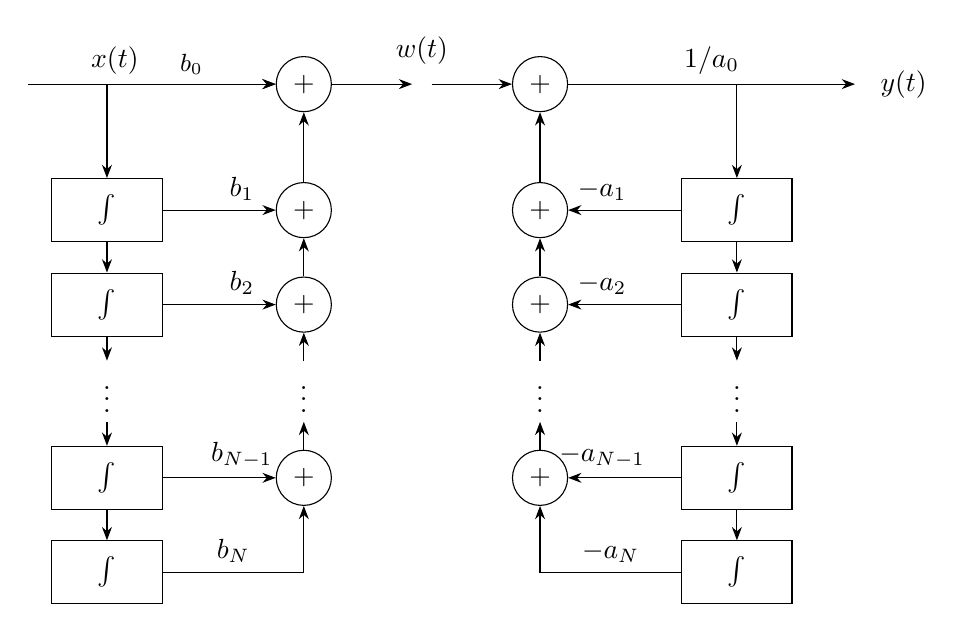
\begin{tikzpicture}[
	node distance=8mm and 18mm,
	block/.style={rectangle, draw, minimum width=14mm, minimum height=8mm, align=center},
	sum/.style={circle, draw, minimum size=7mm, inner sep=0pt},
	coeff/.style={font=\small},
	>={Stealth}
	]
	
	% Main horizontal nodes
	\coordinate (input) at (0,0);
	\node[sum] (feedforward_sum) at (3.5,0) {$+$};
	\node (intermediate_signal) at (5,0) [label=above:{$w(t)$}] {};
	\node[sum] (feedback_sum) at (6.5,0) {$+$};
	\coordinate (output) at (10.5,0);
	
	% Main path arrows and labels
	\draw[->] (input) -- node[above,pos=0.35] {$x(t)$} (feedforward_sum);
	\draw[->] (feedforward_sum) -- (intermediate_signal);
	\draw[->] (intermediate_signal) -- (feedback_sum);
	\draw[->] (feedback_sum) -- node[above] {$1/a_0$} (output) node[right=2mm] {$y(t)$};
	
	%
	% Feedforward column (left)
	%
	% a vertical bus point where taps branch off
	\coordinate (feedforward_bus) at (1,0);
	
	% integrators stacked below ffbus
	\node[block] (int_1) at ($(feedforward_bus)+(0,-1.6)$) {$\int$};
	\node[block] (int_2) at ($(int_1)+(0,-1.2)$) {$\int$};
	\node (int_dots) at ($(int_2)+(0,-1.1)$) {$\vdots$};
	\node[block] (int_N_minus_1) at ($(int_dots)+(0,-1.1)$) {$\int$};
	\node[block] (int_N) at ($(int_N_minus_1)+(0,-1.2)$) {$\int$};
	
	% feedforward bus line and branch to ffsum
	\draw (feedforward_bus) -- ++(0.8,0); % small visual bus
	\draw[->] (feedforward_bus) -- node[above,pos=0.5,coeff] {$b_0$} (feedforward_sum);
	
	% connect the bus to first integrator
	\draw[->] (feedforward_bus) -- (int_1.north);
	
	% chain integrators
	\draw[->] (int_1) -- (int_2);
	\draw[->] (int_2) -- (int_dots);
	\draw[->] (int_dots) -- (int_N_minus_1);
	\draw[->] (int_N_minus_1) -- (int_N);
	
	% summers for each integrated tap
	\node[sum] (sum_1) at ($(feedforward_sum) + (0,-1.6)$) {$+$};
	\node[sum] (sum_2) at ($(sum_1) + (0,-1.2)$) {$+$};
	\node (sum_dots) at ($(sum_2) + (0,-1.1)$) {$\vdots$};
	\node[sum] (sum_N_minus_1) at ($(sum_dots) + (0,-1.1)$) {$+$};
	
	% connections from integrators to the corresponding summers
	\draw[->] (int_1) -- node[above, pos=0.7] {$b_1$} (sum_1);
	\draw[->] (int_2) -- node[above, pos=0.7] {$b_2$} (sum_2);
	\draw[->] (int_N_minus_1) -- node[above, pos=0.7] {$b_{N-1}$} (sum_N_minus_1);
	\draw[->] (int_N) -| (sum_N_minus_1) node[above, pos=0.25] {$b_N$};
	
	% chain the summers into ffsum
	\draw[->] (sum_1) -- (feedforward_sum);
	\draw[->] (sum_2) -- (sum_1);
	\draw[->] (sum_N_minus_1) -- (sum_dots);
	\draw[->] (sum_dots) -- (sum_2);
	
	%
	% Feedback column (right)
	%
	\coordinate (feedback_bus) at (9,0);
	
	\node[block] (feedback_int_1) at ($(feedback_bus)+(0,-1.6)$) {$\int$};
	\node[block] (feedback_int_2) at ($(feedback_int_1)+(0,-1.2)$) {$\int$};
	\node (feedback_int_dots) at ($(feedback_int_2)+(0,-1.1)$) {$\vdots$};
	\node[block] (feedback_int_N_minus_1) at ($(feedback_int_dots)+(0,-1.1)$) {$\int$};
	\node[block] (feedback_int_N) at ($(feedback_int_N_minus_1)+(0,-1.2)$) {$\int$};
	
	% bus line and chain
	\draw (feedback_bus) -- ++(-0.8,0); % small visual bus
	\draw[->] (feedback_bus) -- (feedback_int_1.north);
	\draw[->] (feedback_int_1) -- (feedback_int_2);
	\draw[->] (feedback_int_2) -- (feedback_int_dots);
	\draw[->] (feedback_int_dots) -- (feedback_int_N_minus_1);
	\draw[->] (feedback_int_N_minus_1) -- (feedback_int_N);
	
	% feedback summers
	\node[sum] (feedback_sum_1) at ($(feedback_sum) + (0,-1.6)$) {$+$};
	\node[sum] (feedback_sum_2) at ($(feedback_sum_1) + (0,-1.2)$) {$+$};
	\node (feedback_sum_dots) at ($(feedback_sum_2) + (0,-1.1)$) {$\vdots$};
	\node[sum] (feedback_sum_N_minus_1) at ($(feedback_sum_dots) + (0,-1.1)$) {$+$};
	
	% connections from feedback integrators to feedback summers (with -a_i)
	\draw[->] (feedback_int_1) -- node[above, pos=0.7] {$-a_1$} (feedback_sum_1);
	\draw[->] (feedback_int_2) -- node[above, pos=0.7] {$-a_2$} (feedback_sum_2);
	\draw[->] (feedback_int_N_minus_1) -- node[above, pos=0.7] {$-a_{N-1}$} (feedback_sum_N_minus_1);
	\draw[->] (feedback_int_N) -| (feedback_sum_N_minus_1) node[above, pos=0.25] {$-a_N$};
	
	% chain feedback summers into main feedback summer
	\draw[->] (feedback_sum_1) -- (feedback_sum);
	\draw[->] (feedback_sum_2) -- (feedback_sum_1);
	\draw[->] (feedback_sum_N_minus_1) -- (feedback_sum_dots);
	\draw[->] (feedback_sum_dots) -- (feedback_sum_2);
	
	\end{tikzpicture}
}
	\caption{Direct Form I implementation structure for continuous-time LCCDEs.}
	\label{fig:ct_direct_form_i}
\end{figure}

\begin{figure}[H]
	\centering
	\resizebox{0.6\textwidth}{!}{	\begin{tikzpicture}[
		node distance=10mm and 22mm,
		block/.style={rectangle, draw, minimum width=12mm, minimum height=8mm, align=center},
		sum/.style={circle, draw, minimum size=7mm, inner sep=0pt},
		>={Stealth},
		% Style for placing labels on lines
		coeff/.style={above, pos=0.5}
		]
		
		% --- Main Horizontal Nodes at the Top ---
		\coordinate (input) at (0,0);
		\node[sum] (feedback_sum_top) at (2.5,0) {$+$};
		\coordinate (w_point) at (5,0);
		\node[sum] (feedforward_sum_top) at (7.5,0) {$+$};
		\coordinate (output) at (10,0);
		
		% --- Draw the Top-Level Signal Path ---
		\draw[->] (input) -- node[coeff, pos=0.4] {$x(t)$} (feedback_sum_top);
		\draw[->] (feedback_sum_top) -- (w_point);
		\node[above=2mm] at (w_point) {$w(t)$};
		\draw[->] (w_point) -- node[coeff] {$b_0$} (feedforward_sum_top);
		\draw[->] (feedforward_sum_top) -- node[coeff, pos=0.6] {$y(t)$} (output);
		
		% --- Central Integrator Column ---
		\node[block] (int1) at ($(w_point)+(0,-2.2)$) {$\int$};
		\node[block] (int2) at ($(int1)+(0,-2.2)$) {$\int$};
		\node (dots) at ($(int2)+(0,-1.8)$) {$\vdots$};
		\node[block] (intN_1) at ($(dots)+(0,-1.8)$) {$\int$};
		\node[block] (intN) at ($(intN_1)+(0,-2.2)$) {$\int$};
		
		% --- Vertical Integrator Bus ---
		\draw[->] (w_point) -- (int1);
		\draw[->] (int1) -- (int2);
		\draw[->,shorten >=1mm, shorten <=1mm] (int2) -- (dots);
		\draw[->,shorten >=1mm, shorten <=1mm] (dots) -- (intN_1);
		\draw[->] (intN_1) -- (intN);
		
		% --- Summers on Both Sides ---
		\node[sum] (feedback_sum_1) at (feedback_sum_top |- int1) {$+$};
		\node[sum] (feedback_sum_2) at (feedback_sum_top |- int2) {$+$};
		\node[sum] (feedback_sum_N_1) at (feedback_sum_top |- intN_1) {$+$};
		\node[sum] (feedback_sum_N) at (feedback_sum_top |- intN) {$+$};
		
		\node[sum] (feedforward_sum_1) at (feedforward_sum_top |- int1) {$+$};
		\node[sum] (feedforward_sum_2) at (feedforward_sum_top |- int2) {$+$};
		\node[sum] (feedforward_sum_N_1) at (feedforward_sum_top |- intN_1) {$+$};
		\node[sum] (feedforward_sum_N) at (feedforward_sum_top |- intN) {$+$};
		
			% --- Feedback Connections (Left Side) ---
			% Tap signal from AFTER each integrator block
	% Draw left, place the label, then draw up and over to the destination
		\draw[->] (int1.west) -- ++(-.7,0) node[above] {$-a_1$} |- (feedback_sum_1);
		\draw[->] (int2.west) -- ++(-.7,0) node[above] {$-a_2$} |- (feedback_sum_2);
		\draw[->] (intN_1.west) -- ++(-.7,0) node[above] {$-a_{N-1}$} |- (feedback_sum_N_1);
		\draw[->] (intN.west) -- ++(-.7,0) node[above] {$-a_N$} |- (feedback_sum_N);

		
		% --- Feedforward Connections (Right Side) ---
		% Tap signal from BEFORE each integrator block
		\draw[->] (int1.east) -- ++(.7,0) node[above] {$b_1$} |- (feedforward_sum_1);
		\draw[->] (int2.east) -- ++(.7,0) node[above] {$b_2$} |- (feedforward_sum_2);
		\draw[->] (intN_1.east) -- ++(.7,0) node[above] {$b_{N-1}$} |- (feedforward_sum_N_1);
		\draw[->] (intN.east) -- ++(.7,0) node[above] {$b_N$} |- (feedforward_sum_N);
		
		
		% --- Vertical Summer Connections ---
		% Connect the summers in an upward chain
		\draw[->] (feedback_sum_1) -- (feedback_sum_top);
		\draw[->] (feedback_sum_2) -- (feedback_sum_1);
		\draw[->, dotted] (feedback_sum_N_1) -- (feedback_sum_2);
		\draw[->] (feedback_sum_N) -- (feedback_sum_N_1);
		
		\draw[->] (feedforward_sum_1) -- (feedforward_sum_top);
		\draw[->] (feedforward_sum_2) -- (feedforward_sum_1);
		\draw[->, dotted] (feedforward_sum_N_1) -- (feedforward_sum_2);
		\draw[->] (feedforward_sum_N) -- (feedforward_sum_N_1);
		

	\end{tikzpicture}
}
	\caption{Direct Form II (Canonic) implementation structure for continuous-time LCCDEs.}
	\label{fig:ct_direct_form_ii}
\end{figure}

\subsection*{6.6.3 Key Implementation Considerations}

\textbf{Direct Form I Advantages:}
\begin{itemize}[noitemsep]
	\item Clear separation between feedforward and feedback
	\item Less sensitive to coefficient quantization
	\item Easier to understand and debug
\end{itemize}

\textbf{Direct Form II Advantages:}
\begin{itemize}[noitemsep]
	\item Minimal memory usage (half the delays)
	\item More efficient for high-order systems
	\item Standard in many DSP libraries
\end{itemize}

\textbf{Implementation Challenges:}
\begin{itemize}[noitemsep]
	\item Numerical precision issues with high-order systems
	\item Potential for limit cycles in fixed-point implementations
	\item Need for careful coefficient scaling
\end{itemize}

\section*{6.8 Practical Examples and Applications}

\subsection*{6.8.1 Continuous-Time Examples}

\begin{example}[RLC Circuit - Second Order]
Consider an RLC circuit with input voltage $x(t)$ and output voltage $y(t)$:
\[
L\frac{\dd^2 y}{\dd t^2} + R\frac{\dd y}{\dd t} + \frac{1}{C}y = \frac{\dd x}{\dd t}
\]
This is a second-order system with:
\begin{itemize}[noitemsep]
	\item Natural frequency: $\omega_n = \frac{1}{\sqrt{LC}}$
	\item Damping ratio: $\zeta = \frac{R}{2}\sqrt{\frac{C}{L}}$
	\item Can be underdamped, critically damped, or overdamped
\end{itemize}
\end{example}

\begin{example}[Mechanical System - Mass-Spring-Damper]
Consider a mass-spring-damper system:
\[
m\frac{\dd^2 y}{\dd t^2} + c\frac{\dd y}{\dd t} + ky = x(t)
\]
where $m$ is mass, $c$ is damping coefficient, and $k$ is spring constant.
\end{example}

\subsection*{6.8.2 Discrete-Time Examples}

\begin{example}[Digital Filter Design]
A common digital low-pass filter:
\[
y[n] = 0.1x[n] + 0.9y[n-1]
\]
This is a first-order IIR filter with cutoff frequency determined by the coefficient 0.9.
\end{example}

\begin{example}[Echo Cancellation]
An echo cancellation system:
\[
y[n] = x[n] + \alpha x[n-D] + \beta y[n-D]
\]
where $D$ is the delay, and $\alpha$, $\beta$ are echo parameters.
\end{example}

\subsection*{6.8.3 System Analysis from LCCDEs}

\textbf{Stability Analysis:}
\begin{itemize}[noitemsep]
	\item CT: All poles must be in the left half-plane
	\item DT: All poles must be inside the unit circle
	\item For rational transfer functions, this is equivalent to BIBO stability
\end{itemize}


\begin{remark}
We are only introducing these today. We will spend a significant part of the course developing powerful techniques (Fourier, Laplace, and z-transforms) to solve these equations and analyze the systems they represent. For now, the goal is to recognize their form and their connection to LTI systems under the initial rest condition.
\end{remark}


\section*{6.9 Common Pitfalls and Clarifications}

\begin{itemize}[noitemsep]
	\item \textbf{Initial rest vs linearity:} A system is truly linear if its output is solely the result of the input signal being processed. This relationship, described by pure convolution, only holds if the system starts at rest (with zero stored energy). If a system has nonzero initial conditions, like a charged capacitor, its output is a mix of the response to the input and a response from that initial energy. Because this initial energy response doesn't scale with the input, the overall system no longer behaves linearly.
	\item \textbf{BIBO vs internal stability:} 
	There are two primary ways to judge if a system is stable. The first, called \textbf{BIBO stability}, which is an external ``black-box'' view: if you feed it a well-behaved signal that doesn't go to infinity, you get a well-behaved signal out. The second, \textbf{internal stability}, is an internal ``glass-box'' view that checks if any hidden component within the system will blow up on its own. While it's possible for a system to \textit{appear} stable on the outside while being internally unstable, this isn't a concern for most standard systems we encounter (specifically, \textbf{rational and causal} ones). For these systems, the two types of stability are unified. We only need to check one thing: the \textbf{location of the system's poles}. If all the poles lie in the stable region of the complex plane (the left-half), the system is guaranteed to be stable both inside and out.
	\item \textbf{Memoryless $\neq$ instantaneous hardware:} Differentiators are not memoryless though they "look" instantaneous.
\end{itemize}

\section*{6.10 Quick-Reference Formulas}

\begin{itemize}[noitemsep]
	\item \textbf{Convolution:} CT $y(t) = \int_{-\infty}^{\infty} x(\tau)h(t-\tau)\dd\tau$, DT $y[n] = \sum_{k=-\infty}^{\infty} x[k]h[n-k]$
	\item \textbf{Causality:} $h(t) = 0$ ($t < 0$), $h[n] = 0$ ($n < 0$)
	\item \textbf{BIBO stability:} $\int |h(t)|\dd t < \infty$, $\sum |h[n]| < \infty$
	\item \textbf{Step–impulse link:} $h(t) = \frac{\dd}{\dd t} s(t)$, $h[n] = s[n] - s[n-1]$
	\item \textbf{Correlation:} CT $R_{xy}(t) = \int x(\tau)y(\tau+t)\dd\tau$, DT $R_{xy}[n] = \sum x[k]y[k+n]$
	\item \textbf{Normalized correlation:} CT $\rho_{xy}(t) = \frac{R_{xy}(t)}{\sqrt{R_{xx}(0)R_{yy}(0)}}$, DT $\rho_{xy}[n] = \frac{R_{xy}[n]}{\sqrt{R_{xx}[0]R_{yy}[0]}}$
	\item \textbf{LCCDEs:} CT $\sum a_k y^{(k)} = \sum b_k x^{(k)}$, DT $\sum a_k y[n-k] = \sum b_k x[n-k]$
\end{itemize}
\newpage
\section*{6.11 Summary and Next Lecture}

Today, we have connected the abstract properties of LTI systems to concrete conditions on their impulse responses. This is a critical link between theory and practice. The key takeaways are:
\begin{itemize}[noitemsep]
	\item Causality $\Leftrightarrow h(t)=0$ for $t<0$
	\item Stability $\Leftrightarrow$ the impulse response is absolutely integrable/summable
	\item Convolution properties enable system analysis and design
	\item LCCDEs describe the most important class of practical LTI systems
\end{itemize}

\textbf{Next lecture:} We will begin our journey into Fourier analysis. We will discover that complex exponentials are "eigenfunctions" of LTI systems, a property that turns the difficult operation of convolution into simple multiplication. This will be our first step toward a new, and often much easier, way to analyze signals and systems.

\end{document}
